\documentclass[1p]{elsarticle_modified}
%\bibliographystyle{elsarticle-num}

%\usepackage[colorlinks]{hyperref}
%\usepackage{abbrmath_seonhwa} %\Abb, \Ascr, \Acal ,\Abf, \Afrak
\usepackage{amsfonts}
\usepackage{amssymb}
\usepackage{amsmath}
\usepackage{amsthm}
\usepackage{scalefnt}
\usepackage{amsbsy}
\usepackage{kotex}
\usepackage{caption}
\usepackage{subfig}
\usepackage{color}
\usepackage{graphicx}
\usepackage{xcolor} %% white, black, red, green, blue, cyan, magenta, yellow
\usepackage{float}
\usepackage{setspace}
\usepackage{hyperref}

\usepackage{tikz}
\usetikzlibrary{arrows}

\usepackage{multirow}
\usepackage{array} % fixed length table
\usepackage{hhline}

%%%%%%%%%%%%%%%%%%%%%
\makeatletter
\renewcommand*\env@matrix[1][\arraystretch]{%
	\edef\arraystretch{#1}%
	\hskip -\arraycolsep
	\let\@ifnextchar\new@ifnextchar
	\array{*\c@MaxMatrixCols c}}
\makeatother %https://tex.stackexchange.com/questions/14071/how-can-i-increase-the-line-spacing-in-a-matrix
%%%%%%%%%%%%%%%

\usepackage[normalem]{ulem}

\newcommand{\msout}[1]{\ifmmode\text{\sout{\ensuremath{#1}}}\else\sout{#1}\fi}
%SOURCE: \msout is \stkout macro in https://tex.stackexchange.com/questions/20609/strikeout-in-math-mode

\newcommand{\cancel}[1]{
	\ifmmode
	{\color{red}\msout{#1}}
	\else
	{\color{red}\sout{#1}}
	\fi
}

\newcommand{\add}[1]{
	{\color{blue}\uwave{#1}}
}

\newcommand{\replace}[2]{
	\ifmmode
	{\color{red}\msout{#1}}{\color{blue}\uwave{#2}}
	\else
	{\color{red}\sout{#1}}{\color{blue}\uwave{#2}}
	\fi
}

\newcommand{\Sol}{\mathcal{S}} %segment
\newcommand{\D}{D} %diagram
\newcommand{\A}{\mathcal{A}} %arc


%%%%%%%%%%%%%%%%%%%%%%%%%%%%%5 test

\def\sl{\operatorname{\textup{SL}}(2,\Cbb)}
\def\psl{\operatorname{\textup{PSL}}(2,\Cbb)}
\def\quan{\mkern 1mu \triangleright \mkern 1mu}

\theoremstyle{definition}
\newtheorem{thm}{Theorem}[section]
\newtheorem{prop}[thm]{Proposition}
\newtheorem{lem}[thm]{Lemma}
\newtheorem{ques}[thm]{Question}
\newtheorem{cor}[thm]{Corollary}
\newtheorem{defn}[thm]{Definition}
\newtheorem{exam}[thm]{Example}
\newtheorem{rmk}[thm]{Remark}
\newtheorem{alg}[thm]{Algorithm}

\newcommand{\I}{\sqrt{-1}}
\begin{document}

%\begin{frontmatter}
%
%\title{Boundary parabolic representations of knots up to 8 crossings}
%
%%% Group authors per affiliation:
%\author{Yunhi Cho} 
%\address{Department of Mathematics, University of Seoul, Seoul, Korea}
%\ead{yhcho@uos.ac.kr}
%
%
%\author{Seonhwa Kim} %\fnref{s_kim}}
%\address{Center for Geometry and Physics, Institute for Basic Science, Pohang, 37673, Korea}
%\ead{ryeona17@ibs.re.kr}
%
%\author{Hyuk Kim}
%\address{Department of Mathematical Sciences, Seoul National University, Seoul 08826, Korea}
%\ead{hyukkim@snu.ac.kr}
%
%\author{Seokbeom Yoon}
%\address{Department of Mathematical Sciences, Seoul National University, Seoul, 08826,  Korea}
%\ead{sbyoon15@snu.ac.kr}
%
%\begin{abstract}
%We find all boundary parabolic representation of knots up to 8 crossings.
%
%\end{abstract}
%\begin{keyword}
%    \MSC[2010] 57M25 
%\end{keyword}
%
%\end{frontmatter}

%\linenumbers
%\tableofcontents
%
\newcommand\colored[1]{\textcolor{white}{\rule[-0.35ex]{0.8em}{1.4ex}}\kern-0.8em\color{red} #1}%
%\newcommand\colored[1]{\textcolor{white}{ #1}\kern-2.17ex	\textcolor{white}{ #1}\kern-1.81ex	\textcolor{white}{ #1}\kern-2.15ex\color{red}#1	}

{\Large $\underline{12a_{0135}~(K12a_{0135})}$}

\setlength{\tabcolsep}{10pt}
\renewcommand{\arraystretch}{1.6}
\vspace{1cm}\begin{tabular}{m{100pt}>{\centering\arraybackslash}m{274pt}}
\multirow{5}{120pt}{
	\centering
	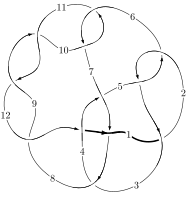
\includegraphics[width=112pt]{../../../GIT/diagram.site/Diagrams/png/936_12a_0135.png}\\
\ \ \ A knot diagram\footnotemark}&
\allowdisplaybreaks
\textbf{Linearized knot diagam} \\
\cline{2-2}
 &
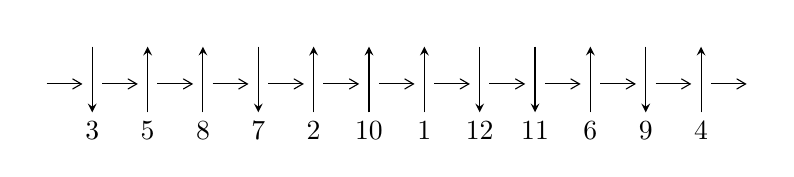
\begin{tikzpicture}[x=20pt, y=17pt]
	% nodes
	\node (C0) at (0, 0) {};
	\node (C1) at (1, 0) {};
	\node (C1U) at (1, +1) {};
	\node (C1D) at (1, -1) {3};

	\node (C2) at (2, 0) {};
	\node (C2U) at (2, +1) {};
	\node (C2D) at (2, -1) {5};

	\node (C3) at (3, 0) {};
	\node (C3U) at (3, +1) {};
	\node (C3D) at (3, -1) {8};

	\node (C4) at (4, 0) {};
	\node (C4U) at (4, +1) {};
	\node (C4D) at (4, -1) {7};

	\node (C5) at (5, 0) {};
	\node (C5U) at (5, +1) {};
	\node (C5D) at (5, -1) {2};

	\node (C6) at (6, 0) {};
	\node (C6U) at (6, +1) {};
	\node (C6D) at (6, -1) {10};

	\node (C7) at (7, 0) {};
	\node (C7U) at (7, +1) {};
	\node (C7D) at (7, -1) {1};

	\node (C8) at (8, 0) {};
	\node (C8U) at (8, +1) {};
	\node (C8D) at (8, -1) {12};

	\node (C9) at (9, 0) {};
	\node (C9U) at (9, +1) {};
	\node (C9D) at (9, -1) {11};

	\node (C10) at (10, 0) {};
	\node (C10U) at (10, +1) {};
	\node (C10D) at (10, -1) {6};

	\node (C11) at (11, 0) {};
	\node (C11U) at (11, +1) {};
	\node (C11D) at (11, -1) {9};

	\node (C12) at (12, 0) {};
	\node (C12U) at (12, +1) {};
	\node (C12D) at (12, -1) {4};
	\node (C13) at (13, 0) {};

	% arrows
	\draw[->,>={angle 60}]
	(C0) edge (C1) (C1) edge (C2) (C2) edge (C3) (C3) edge (C4) (C4) edge (C5) (C5) edge (C6) (C6) edge (C7) (C7) edge (C8) (C8) edge (C9) (C9) edge (C10) (C10) edge (C11) (C11) edge (C12) (C12) edge (C13) ;	\draw[->,>=stealth]
	(C1U) edge (C1D) (C2D) edge (C2U) (C3D) edge (C3U) (C4U) edge (C4D) (C5D) edge (C5U) (C6D) edge (C6U) (C7D) edge (C7U) (C8U) edge (C8D) (C9U) edge (C9D) (C10D) edge (C10U) (C11U) edge (C11D) (C12D) edge (C12U) ;
	\end{tikzpicture} \\
\hhline{~~} \\& 
\textbf{Solving Sequence} \\ \cline{2-2} 
 &
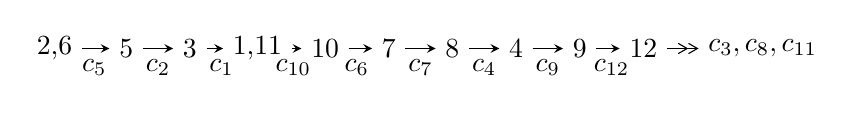
\begin{tikzpicture}[x=23pt, y=7pt]
	% node
	\node (A0) at (-1/8, 0) {2,6};
	\node (A1) at (1, 0) {5};
	\node (A2) at (2, 0) {3};
	\node (A3) at (49/16, 0) {1,11};
	\node (A4) at (33/8, 0) {10};
	\node (A5) at (41/8, 0) {7};
	\node (A6) at (49/8, 0) {8};
	\node (A7) at (57/8, 0) {4};
	\node (A8) at (65/8, 0) {9};
	\node (A9) at (73/8, 0) {12};
	\node (C1) at (1/2, -1) {$c_{5}$};
	\node (C2) at (3/2, -1) {$c_{2}$};
	\node (C3) at (5/2, -1) {$c_{1}$};
	\node (C4) at (29/8, -1) {$c_{10}$};
	\node (C5) at (37/8, -1) {$c_{6}$};
	\node (C6) at (45/8, -1) {$c_{7}$};
	\node (C7) at (53/8, -1) {$c_{4}$};
	\node (C8) at (61/8, -1) {$c_{9}$};
	\node (C9) at (69/8, -1) {$c_{12}$};
	\node (A10) at (11, 0) {$c_{3},c_{8},c_{11}$};

	% edge
	\draw[->,>=stealth]	
	(A0) edge (A1) (A1) edge (A2) (A2) edge (A3) (A3) edge (A4) (A4) edge (A5) (A5) edge (A6) (A6) edge (A7) (A7) edge (A8) (A8) edge (A9) ;
	\draw[->>,>={angle 60}]	
	(A9) edge (A10);
\end{tikzpicture} \\ 

\end{tabular} \\

\footnotetext{
The image of knot diagram is generated by the software ``\textbf{Draw programme}" developed by Andrew Bartholomew(\url{http://www.layer8.co.uk/maths/draw/index.htm\#Running-draw}), where we modified some parts for our purpose(\url{https://github.com/CATsTAILs/LinksPainter}).
}\phantom \\ \newline 
\centering \textbf{Ideals for irreducible components\footnotemark of $X_{\text{par}}$} 
 
\begin{align*}
I^u_{1}&=\langle 
-1.72692\times10^{119} u^{90}-4.57225\times10^{119} u^{89}+\cdots+9.30165\times10^{118} b+8.53692\times10^{118},\\
\phantom{I^u_{1}}&\phantom{= \langle  }-2.15215\times10^{118} u^{90}+2.31866\times10^{118} u^{89}+\cdots+9.30165\times10^{118} a+4.34610\times10^{119},\\
\phantom{I^u_{1}}&\phantom{= \langle  }u^{91}+3 u^{90}+\cdots+6 u-1\rangle \\
I^u_{2}&=\langle 
b+u,\;a- u+3,\;u^2- u+1\rangle \\
I^u_{3}&=\langle 
b- u+1,\;a+1,\;u^2- u+1\rangle \\
\\
\end{align*}
\raggedright * 3 irreducible components of $\dim_{\mathbb{C}}=0$, with total 95 representations.\\
\footnotetext{All coefficients of polynomials are rational numbers. But the coefficients are sometimes approximated in decimal forms when there is not enough margin.}
\newpage
\renewcommand{\arraystretch}{1}
\centering \section*{I. $I^u_{1}= \langle -1.73\times10^{119} u^{90}-4.57\times10^{119} u^{89}+\cdots+9.30\times10^{118} b+8.54\times10^{118},\;-2.15\times10^{118} u^{90}+2.32\times10^{118} u^{89}+\cdots+9.30\times10^{118} a+4.35\times10^{119},\;u^{91}+3 u^{90}+\cdots+6 u-1 \rangle$}
\flushleft \textbf{(i) Arc colorings}\\
\begin{tabular}{m{7pt} m{180pt} m{7pt} m{180pt} }
\flushright $a_{2}=$&$\begin{pmatrix}0\\u\end{pmatrix}$ \\
\flushright $a_{6}=$&$\begin{pmatrix}1\\0\end{pmatrix}$ \\
\flushright $a_{5}=$&$\begin{pmatrix}1\\u^2\end{pmatrix}$ \\
\flushright $a_{3}=$&$\begin{pmatrix}u\\u^3+u\end{pmatrix}$ \\
\flushright $a_{1}=$&$\begin{pmatrix}u^3\\u^5+u^3+u\end{pmatrix}$ \\
\flushright $a_{11}=$&$\begin{pmatrix}0.231373 u^{90}-0.249274 u^{89}+\cdots+24.4495 u-4.67240\\1.85658 u^{90}+4.91553 u^{89}+\cdots+13.7608 u-0.917786\end{pmatrix}$ \\
\flushright $a_{10}=$&$\begin{pmatrix}-1.62521 u^{90}-5.16481 u^{89}+\cdots+10.6888 u-3.75462\\1.85658 u^{90}+4.91553 u^{89}+\cdots+13.7608 u-0.917786\end{pmatrix}$ \\
\flushright $a_{7}=$&$\begin{pmatrix}0.458050 u^{90}+3.21372 u^{89}+\cdots+32.7962 u+1.43676\\-2.25080 u^{90}-6.04356 u^{89}+\cdots-19.0753 u+2.63567\end{pmatrix}$ \\
\flushright $a_{8}=$&$\begin{pmatrix}-4.09748 u^{90}-7.94122 u^{89}+\cdots+15.9952 u+4.35003\\-4.11933 u^{90}-11.4435 u^{89}+\cdots-31.3514 u+4.60999\end{pmatrix}$ \\
\flushright $a_{4}=$&$\begin{pmatrix}-0.0190941 u^{90}+0.310953 u^{89}+\cdots+23.5765 u-3.48020\\-1.31966 u^{90}-2.74606 u^{89}+\cdots+8.20849 u-0.608729\end{pmatrix}$ \\
\flushright $a_{9}=$&$\begin{pmatrix}-0.121914 u^{90}-0.846999 u^{89}+\cdots-17.1093 u-3.46520\\0.988446 u^{90}+2.53453 u^{89}+\cdots+11.9943 u-1.32525\end{pmatrix}$ \\
\flushright $a_{12}=$&$\begin{pmatrix}-1.53320 u^{90}-3.62439 u^{89}+\cdots-4.26452 u-0.301799\\-1.15828 u^{90}-3.43455 u^{89}+\cdots-0.939083 u+0.245751\end{pmatrix}$\\&\end{tabular}
\flushleft \textbf{(ii) Obstruction class $= -1$}\\~\\
\flushleft \textbf{(iii) Cusp Shapes $= 0.0831505 u^{90}+2.13230 u^{89}+\cdots-61.4353 u+6.79727$}\\~\\
\newpage\renewcommand{\arraystretch}{1}
\flushleft \textbf{(iv) u-Polynomials at the component}\newline \\
\begin{tabular}{m{50pt}|m{274pt}}
Crossings & \hspace{64pt}u-Polynomials at each crossing \\
\hline $$\begin{aligned}c_{1}\end{aligned}$$&$\begin{aligned}
&u^{91}+33 u^{90}+\cdots-118 u-1
\end{aligned}$\\
\hline $$\begin{aligned}c_{2},c_{5}\end{aligned}$$&$\begin{aligned}
&u^{91}+3 u^{90}+\cdots+6 u-1
\end{aligned}$\\
\hline $$\begin{aligned}c_{3}\end{aligned}$$&$\begin{aligned}
&u^{91}-2 u^{90}+\cdots-13743 u-1847
\end{aligned}$\\
\hline $$\begin{aligned}c_{4}\end{aligned}$$&$\begin{aligned}
&u^{91}-4 u^{90}+\cdots-2610301 u-1139239
\end{aligned}$\\
\hline $$\begin{aligned}c_{6},c_{10}\end{aligned}$$&$\begin{aligned}
&u^{91}-3 u^{90}+\cdots+8 u-1
\end{aligned}$\\
\hline $$\begin{aligned}c_{7}\end{aligned}$$&$\begin{aligned}
&u^{91}+7 u^{90}+\cdots+u^2-1
\end{aligned}$\\
\hline $$\begin{aligned}c_{8},c_{9},c_{11}\end{aligned}$$&$\begin{aligned}
&u^{91}+21 u^{90}+\cdots+2 u-1
\end{aligned}$\\
\hline $$\begin{aligned}c_{12}\end{aligned}$$&$\begin{aligned}
&u^{91}+9 u^{90}+\cdots-48 u-16
\end{aligned}$\\
\hline
\end{tabular}\\~\\
\newpage\renewcommand{\arraystretch}{1}
\flushleft \textbf{(v) Riley Polynomials at the component}\newline \\
\begin{tabular}{m{50pt}|m{274pt}}
Crossings & \hspace{64pt}Riley Polynomials at each crossing \\
\hline $$\begin{aligned}c_{1}\end{aligned}$$&$\begin{aligned}
&y^{91}+53 y^{90}+\cdots+3722 y-1
\end{aligned}$\\
\hline $$\begin{aligned}c_{2},c_{5}\end{aligned}$$&$\begin{aligned}
&y^{91}+33 y^{90}+\cdots-118 y-1
\end{aligned}$\\
\hline $$\begin{aligned}c_{3}\end{aligned}$$&$\begin{aligned}
&y^{91}-126 y^{90}+\cdots+130933353 y-3411409
\end{aligned}$\\
\hline $$\begin{aligned}c_{4}\end{aligned}$$&$\begin{aligned}
&y^{91}-58 y^{90}+\cdots-17761718980039 y-1297865499121
\end{aligned}$\\
\hline $$\begin{aligned}c_{6},c_{10}\end{aligned}$$&$\begin{aligned}
&y^{91}+21 y^{90}+\cdots+2 y-1
\end{aligned}$\\
\hline $$\begin{aligned}c_{7}\end{aligned}$$&$\begin{aligned}
&y^{91}-7 y^{90}+\cdots+2 y-1
\end{aligned}$\\
\hline $$\begin{aligned}c_{8},c_{9},c_{11}\end{aligned}$$&$\begin{aligned}
&y^{91}+101 y^{90}+\cdots-174 y-1
\end{aligned}$\\
\hline $$\begin{aligned}c_{12}\end{aligned}$$&$\begin{aligned}
&y^{91}-25 y^{90}+\cdots+1664 y-256
\end{aligned}$\\
\hline
\end{tabular}\\~\\
\newpage\flushleft \textbf{(vi) Complex Volumes and Cusp Shapes}
$$\begin{array}{c|c|c}  
\text{Solutions to }I^u_{1}& \I (\text{vol} + \sqrt{-1}CS) & \text{Cusp shape}\\
 \hline 
\begin{aligned}
u &= -0.849901 + 0.532640 I \\
a &= -0.963557 - 0.039990 I \\
b &= -0.501919 - 0.972635 I\end{aligned}
 & \phantom{-}2.60124 + 7.64482 I & \phantom{-0.000000 } 0 \\ \hline\begin{aligned}
u &= -0.849901 - 0.532640 I \\
a &= -0.963557 + 0.039990 I \\
b &= -0.501919 + 0.972635 I\end{aligned}
 & \phantom{-}2.60124 - 7.64482 I & \phantom{-0.000000 } 0 \\ \hline\begin{aligned}
u &= -0.817325 + 0.615518 I \\
a &= -1.232520 + 0.074616 I \\
b &= -0.740788 + 0.415458 I\end{aligned}
 & \phantom{-}4.41799 + 3.11359 I & \phantom{-0.000000 } 0 \\ \hline\begin{aligned}
u &= -0.817325 - 0.615518 I \\
a &= -1.232520 - 0.074616 I \\
b &= -0.740788 - 0.415458 I\end{aligned}
 & \phantom{-}4.41799 - 3.11359 I & \phantom{-0.000000 } 0 \\ \hline\begin{aligned}
u &= \phantom{-}0.519619 + 0.884274 I \\
a &= \phantom{-}5.36046 - 1.09932 I \\
b &= \phantom{-}0.388031 + 0.748802 I\end{aligned}
 & -0.12886 + 3.65979 I & \phantom{-0.000000 } 0 \\ \hline\begin{aligned}
u &= \phantom{-}0.519619 - 0.884274 I \\
a &= \phantom{-}5.36046 + 1.09932 I \\
b &= \phantom{-}0.388031 - 0.748802 I\end{aligned}
 & -0.12886 - 3.65979 I & \phantom{-0.000000 } 0 \\ \hline\begin{aligned}
u &= \phantom{-}0.510616 + 0.827287 I \\
a &= \phantom{-}2.72439 - 2.64972 I \\
b &= \phantom{-}0.405786 - 0.690615 I\end{aligned}
 & \phantom{-}0.060399 + 0.518242 I & \phantom{-0.000000 } 0 \\ \hline\begin{aligned}
u &= \phantom{-}0.510616 - 0.827287 I \\
a &= \phantom{-}2.72439 + 2.64972 I \\
b &= \phantom{-}0.405786 + 0.690615 I\end{aligned}
 & \phantom{-}0.060399 - 0.518242 I & \phantom{-0.000000 } 0 \\ \hline\begin{aligned}
u &= -0.692631 + 0.759883 I \\
a &= \phantom{-}0.656579 + 0.844041 I \\
b &= \phantom{-}0.770775 + 0.266041 I\end{aligned}
 & \phantom{-}3.68029 + 0.01829 I & \phantom{-0.000000 } 0 \\ \hline\begin{aligned}
u &= -0.692631 - 0.759883 I \\
a &= \phantom{-}0.656579 - 0.844041 I \\
b &= \phantom{-}0.770775 - 0.266041 I\end{aligned}
 & \phantom{-}3.68029 - 0.01829 I & \phantom{-0.000000 } 0\\
 \hline 
 \end{array}$$\newpage$$\begin{array}{c|c|c}  
\text{Solutions to }I^u_{1}& \I (\text{vol} + \sqrt{-1}CS) & \text{Cusp shape}\\
 \hline 
\begin{aligned}
u &= -0.617883 + 0.826016 I \\
a &= \phantom{-}1.83951 + 0.89847 I \\
b &= \phantom{-}0.426311 - 1.065410 I\end{aligned}
 & \phantom{-}1.05247 - 4.32716 I & \phantom{-0.000000 } 0 \\ \hline\begin{aligned}
u &= -0.617883 - 0.826016 I \\
a &= \phantom{-}1.83951 - 0.89847 I \\
b &= \phantom{-}0.426311 + 1.065410 I\end{aligned}
 & \phantom{-}1.05247 + 4.32716 I & \phantom{-0.000000 } 0 \\ \hline\begin{aligned}
u &= -0.726000 + 0.745604 I \\
a &= -1.29706 - 0.82696 I \\
b &= -0.872823 - 0.989713 I\end{aligned}
 & \phantom{-}10.44210 + 3.74493 I & \phantom{-0.000000 } 0 \\ \hline\begin{aligned}
u &= -0.726000 - 0.745604 I \\
a &= -1.29706 + 0.82696 I \\
b &= -0.872823 + 0.989713 I\end{aligned}
 & \phantom{-}10.44210 - 3.74493 I & \phantom{-0.000000 } 0 \\ \hline\begin{aligned}
u &= \phantom{-}0.602511 + 0.853945 I \\
a &= -0.234195 + 0.139093 I \\
b &= \phantom{-}0.230041 + 0.140089 I\end{aligned}
 & \phantom{-}0.59146 + 2.37151 I & \phantom{-0.000000 } 0 \\ \hline\begin{aligned}
u &= \phantom{-}0.602511 - 0.853945 I \\
a &= -0.234195 - 0.139093 I \\
b &= \phantom{-}0.230041 - 0.140089 I\end{aligned}
 & \phantom{-}0.59146 - 2.37151 I & \phantom{-0.000000 } 0 \\ \hline\begin{aligned}
u &= \phantom{-}0.599752 + 0.859541 I \\
a &= -1.43361 + 3.11843 I \\
b &= -0.863708 + 0.907500 I\end{aligned}
 & \phantom{-}7.32016 - 0.83535 I & \phantom{-0.000000 } 0 \\ \hline\begin{aligned}
u &= \phantom{-}0.599752 - 0.859541 I \\
a &= -1.43361 - 3.11843 I \\
b &= -0.863708 - 0.907500 I\end{aligned}
 & \phantom{-}7.32016 + 0.83535 I & \phantom{-0.000000 } 0 \\ \hline\begin{aligned}
u &= \phantom{-}0.877497 + 0.363830 I \\
a &= -1.038190 - 0.060966 I \\
b &= -0.508067 + 0.669065 I\end{aligned}
 & \phantom{-}2.84624 - 0.28140 I & \phantom{-0.000000 } 0 \\ \hline\begin{aligned}
u &= \phantom{-}0.877497 - 0.363830 I \\
a &= -1.038190 + 0.060966 I \\
b &= -0.508067 - 0.669065 I\end{aligned}
 & \phantom{-}2.84624 + 0.28140 I & \phantom{-0.000000 } 0\\
 \hline 
 \end{array}$$\newpage$$\begin{array}{c|c|c}  
\text{Solutions to }I^u_{1}& \I (\text{vol} + \sqrt{-1}CS) & \text{Cusp shape}\\
 \hline 
\begin{aligned}
u &= \phantom{-}0.431094 + 0.846214 I \\
a &= -1.09578 + 3.27982 I \\
b &= \phantom{-}0.259700 - 0.740101 I\end{aligned}
 & -0.645516 + 0.537865 I & \phantom{-0.000000 } 0 \\ \hline\begin{aligned}
u &= \phantom{-}0.431094 - 0.846214 I \\
a &= -1.09578 - 3.27982 I \\
b &= \phantom{-}0.259700 + 0.740101 I\end{aligned}
 & -0.645516 - 0.537865 I & \phantom{-0.000000 } 0 \\ \hline\begin{aligned}
u &= \phantom{-}0.596746 + 0.874010 I \\
a &= -4.24870 - 0.23202 I \\
b &= -0.857433 - 0.922091 I\end{aligned}
 & \phantom{-}7.27361 + 5.54804 I & \phantom{-0.000000 } 0 \\ \hline\begin{aligned}
u &= \phantom{-}0.596746 - 0.874010 I \\
a &= -4.24870 + 0.23202 I \\
b &= -0.857433 + 0.922091 I\end{aligned}
 & \phantom{-}7.27361 - 5.54804 I & \phantom{-0.000000 } 0 \\ \hline\begin{aligned}
u &= \phantom{-}0.894016 + 0.581594 I \\
a &= -1.121050 + 0.001326 I \\
b &= -0.496497 - 0.735231 I\end{aligned}
 & \phantom{-}2.63988 + 3.58113 I & \phantom{-0.000000 } 0 \\ \hline\begin{aligned}
u &= \phantom{-}0.894016 - 0.581594 I \\
a &= -1.121050 - 0.001326 I \\
b &= -0.496497 + 0.735231 I\end{aligned}
 & \phantom{-}2.63988 - 3.58113 I & \phantom{-0.000000 } 0 \\ \hline\begin{aligned}
u &= -0.733854 + 0.776716 I \\
a &= -1.82619 + 0.31741 I \\
b &= -0.934033 + 0.867541 I\end{aligned}
 & \phantom{-}10.83630 - 2.90148 I & \phantom{-0.000000 } 0 \\ \hline\begin{aligned}
u &= -0.733854 - 0.776716 I \\
a &= -1.82619 - 0.31741 I \\
b &= -0.934033 - 0.867541 I\end{aligned}
 & \phantom{-}10.83630 + 2.90148 I & \phantom{-0.000000 } 0 \\ \hline\begin{aligned}
u &= -0.280961 + 0.884040 I \\
a &= \phantom{-}2.09555 + 1.09791 I \\
b &= \phantom{-}0.647761 - 0.936156 I\end{aligned}
 & -1.00500 - 3.64630 I & \phantom{-0.000000 } 0 \\ \hline\begin{aligned}
u &= -0.280961 - 0.884040 I \\
a &= \phantom{-}2.09555 - 1.09791 I \\
b &= \phantom{-}0.647761 + 0.936156 I\end{aligned}
 & -1.00500 + 3.64630 I & \phantom{-0.000000 } 0\\
 \hline 
 \end{array}$$\newpage$$\begin{array}{c|c|c}  
\text{Solutions to }I^u_{1}& \I (\text{vol} + \sqrt{-1}CS) & \text{Cusp shape}\\
 \hline 
\begin{aligned}
u &= \phantom{-}0.112513 + 1.073590 I \\
a &= -0.327040 - 0.315830 I \\
b &= -0.504186 + 0.242565 I\end{aligned}
 & -1.94008 + 2.47820 I & \phantom{-0.000000 } 0 \\ \hline\begin{aligned}
u &= \phantom{-}0.112513 - 1.073590 I \\
a &= -0.327040 + 0.315830 I \\
b &= -0.504186 - 0.242565 I\end{aligned}
 & -1.94008 - 2.47820 I & \phantom{-0.000000 } 0 \\ \hline\begin{aligned}
u &= -0.093647 + 1.075460 I \\
a &= -0.92238 - 1.67542 I \\
b &= -0.116466 + 0.924714 I\end{aligned}
 & -5.30788 + 0.87494 I & \phantom{-0.000000 } 0 \\ \hline\begin{aligned}
u &= -0.093647 - 1.075460 I \\
a &= -0.92238 + 1.67542 I \\
b &= -0.116466 - 0.924714 I\end{aligned}
 & -5.30788 - 0.87494 I & \phantom{-0.000000 } 0 \\ \hline\begin{aligned}
u &= -0.612905 + 0.889404 I \\
a &= \phantom{-}0.290577 - 0.103085 I \\
b &= \phantom{-}0.499503 + 1.060910 I\end{aligned}
 & \phantom{-}0.851704 - 0.510059 I & \phantom{-0.000000 } 0 \\ \hline\begin{aligned}
u &= -0.612905 - 0.889404 I \\
a &= \phantom{-}0.290577 + 0.103085 I \\
b &= \phantom{-}0.499503 - 1.060910 I\end{aligned}
 & \phantom{-}0.851704 + 0.510059 I & \phantom{-0.000000 } 0 \\ \hline\begin{aligned}
u &= \phantom{-}0.184750 + 0.886590 I \\
a &= \phantom{-}0.13634 - 1.47179 I \\
b &= -0.836064 + 0.881099 I\end{aligned}
 & \phantom{-}5.34127 - 1.26788 I & \phantom{-0.000000 } 0 \\ \hline\begin{aligned}
u &= \phantom{-}0.184750 - 0.886590 I \\
a &= \phantom{-}0.13634 + 1.47179 I \\
b &= -0.836064 - 0.881099 I\end{aligned}
 & \phantom{-}5.34127 + 1.26788 I & \phantom{-0.000000 } 0 \\ \hline\begin{aligned}
u &= \phantom{-}0.131289 + 0.875525 I \\
a &= \phantom{-}0.360689 + 1.151290 I \\
b &= -0.819487 - 0.926120 I\end{aligned}
 & \phantom{-}5.19890 + 4.91121 I & \phantom{-0.000000 } 0 \\ \hline\begin{aligned}
u &= \phantom{-}0.131289 - 0.875525 I \\
a &= \phantom{-}0.360689 - 1.151290 I \\
b &= -0.819487 + 0.926120 I\end{aligned}
 & \phantom{-}5.19890 - 4.91121 I & \phantom{-0.000000 } 0\\
 \hline 
 \end{array}$$\newpage$$\begin{array}{c|c|c}  
\text{Solutions to }I^u_{1}& \I (\text{vol} + \sqrt{-1}CS) & \text{Cusp shape}\\
 \hline 
\begin{aligned}
u &= -0.970603 + 0.569422 I \\
a &= \phantom{-}1.70225 + 0.58793 I \\
b &= \phantom{-}0.861320 + 0.981783 I\end{aligned}
 & \phantom{-}11.5861 + 11.3303 I & \phantom{-0.000000 } 0 \\ \hline\begin{aligned}
u &= -0.970603 - 0.569422 I \\
a &= \phantom{-}1.70225 - 0.58793 I \\
b &= \phantom{-}0.861320 - 0.981783 I\end{aligned}
 & \phantom{-}11.5861 - 11.3303 I & \phantom{-0.000000 } 0 \\ \hline\begin{aligned}
u &= -0.963311 + 0.587822 I \\
a &= \phantom{-}1.64789 - 0.70694 I \\
b &= \phantom{-}0.917846 - 0.864762 I\end{aligned}
 & \phantom{-}11.96280 + 4.76976 I & \phantom{-0.000000 } 0 \\ \hline\begin{aligned}
u &= -0.963311 - 0.587822 I \\
a &= \phantom{-}1.64789 + 0.70694 I \\
b &= \phantom{-}0.917846 + 0.864762 I\end{aligned}
 & \phantom{-}11.96280 - 4.76976 I & \phantom{-0.000000 } 0 \\ \hline\begin{aligned}
u &= \phantom{-}0.456158 + 1.037480 I \\
a &= -0.389843 - 1.240120 I \\
b &= -0.031963 + 0.662712 I\end{aligned}
 & -1.30740 + 2.81413 I & \phantom{-0.000000 } 0 \\ \hline\begin{aligned}
u &= \phantom{-}0.456158 - 1.037480 I \\
a &= -0.389843 + 1.240120 I \\
b &= -0.031963 - 0.662712 I\end{aligned}
 & -1.30740 - 2.81413 I & \phantom{-0.000000 } 0 \\ \hline\begin{aligned}
u &= -0.616797 + 0.586810 I \\
a &= -0.630115 - 0.593051 I \\
b &= \phantom{-}0.091943 + 1.003370 I\end{aligned}
 & -0.77636 + 2.15470 I & \phantom{-0.000000 } 0. - 4.37699 I \\ \hline\begin{aligned}
u &= -0.616797 - 0.586810 I \\
a &= -0.630115 + 0.593051 I \\
b &= \phantom{-}0.091943 - 1.003370 I\end{aligned}
 & -0.77636 - 2.15470 I & \phantom{-0.000000 -}0. + 4.37699 I \\ \hline\begin{aligned}
u &= -0.669127 + 0.933812 I \\
a &= \phantom{-}1.053490 + 0.257114 I \\
b &= \phantom{-}0.805821 - 0.356822 I\end{aligned}
 & \phantom{-}3.14957 - 5.27168 I & \phantom{-0.000000 } 0 \\ \hline\begin{aligned}
u &= -0.669127 - 0.933812 I \\
a &= \phantom{-}1.053490 - 0.257114 I \\
b &= \phantom{-}0.805821 + 0.356822 I\end{aligned}
 & \phantom{-}3.14957 + 5.27168 I & \phantom{-0.000000 } 0\\
 \hline 
 \end{array}$$\newpage$$\begin{array}{c|c|c}  
\text{Solutions to }I^u_{1}& \I (\text{vol} + \sqrt{-1}CS) & \text{Cusp shape}\\
 \hline 
\begin{aligned}
u &= -0.709401 + 0.929341 I \\
a &= -0.43176 - 1.36082 I \\
b &= -0.933066 - 0.835236 I\end{aligned}
 & \phantom{-}10.37540 - 2.59766 I & \phantom{-0.000000 } 0 \\ \hline\begin{aligned}
u &= -0.709401 - 0.929341 I \\
a &= -0.43176 + 1.36082 I \\
b &= -0.933066 + 0.835236 I\end{aligned}
 & \phantom{-}10.37540 + 2.59766 I & \phantom{-0.000000 } 0 \\ \hline\begin{aligned}
u &= -0.692398 + 0.948673 I \\
a &= -2.37573 - 0.68073 I \\
b &= -0.851462 + 1.006150 I\end{aligned}
 & \phantom{-}9.82767 - 9.16908 I & \phantom{-0.000000 } 0 \\ \hline\begin{aligned}
u &= -0.692398 - 0.948673 I \\
a &= -2.37573 + 0.68073 I \\
b &= -0.851462 - 1.006150 I\end{aligned}
 & \phantom{-}9.82767 + 9.16908 I & \phantom{-0.000000 } 0 \\ \hline\begin{aligned}
u &= -0.623895 + 1.011700 I \\
a &= \phantom{-}0.785245 + 0.975928 I \\
b &= \phantom{-}0.015722 - 1.059090 I\end{aligned}
 & -2.01032 - 7.11313 I & \phantom{-0.000000 } 0 \\ \hline\begin{aligned}
u &= -0.623895 - 1.011700 I \\
a &= \phantom{-}0.785245 - 0.975928 I \\
b &= \phantom{-}0.015722 + 1.059090 I\end{aligned}
 & -2.01032 + 7.11313 I & \phantom{-0.000000 } 0 \\ \hline\begin{aligned}
u &= \phantom{-}0.045555 + 1.214720 I \\
a &= -0.484074 + 1.318660 I \\
b &= -0.393566 - 0.910947 I\end{aligned}
 & -3.80581 + 5.86634 I & \phantom{-0.000000 } 0 \\ \hline\begin{aligned}
u &= \phantom{-}0.045555 - 1.214720 I \\
a &= -0.484074 - 1.318660 I \\
b &= -0.393566 + 0.910947 I\end{aligned}
 & -3.80581 - 5.86634 I & \phantom{-0.000000 } 0 \\ \hline\begin{aligned}
u &= \phantom{-}1.123530 + 0.473437 I \\
a &= \phantom{-}1.55666 - 0.70599 I \\
b &= \phantom{-}0.876538 - 0.914912 I\end{aligned}
 & \phantom{-}10.72650 - 1.33898 I & \phantom{-0.000000 } 0 \\ \hline\begin{aligned}
u &= \phantom{-}1.123530 - 0.473437 I \\
a &= \phantom{-}1.55666 + 0.70599 I \\
b &= \phantom{-}0.876538 + 0.914912 I\end{aligned}
 & \phantom{-}10.72650 + 1.33898 I & \phantom{-0.000000 } 0\\
 \hline 
 \end{array}$$\newpage$$\begin{array}{c|c|c}  
\text{Solutions to }I^u_{1}& \I (\text{vol} + \sqrt{-1}CS) & \text{Cusp shape}\\
 \hline 
\begin{aligned}
u &= \phantom{-}1.120930 + 0.505165 I \\
a &= \phantom{-}1.76081 + 0.51486 I \\
b &= \phantom{-}0.871819 + 0.925682 I\end{aligned}
 & \phantom{-}10.69210 + 5.13030 I & \phantom{-0.000000 } 0 \\ \hline\begin{aligned}
u &= \phantom{-}1.120930 - 0.505165 I \\
a &= \phantom{-}1.76081 - 0.51486 I \\
b &= \phantom{-}0.871819 - 0.925682 I\end{aligned}
 & \phantom{-}10.69210 - 5.13030 I & \phantom{-0.000000 } 0 \\ \hline\begin{aligned}
u &= -0.168598 + 0.743687 I \\
a &= \phantom{-}0.097075 + 1.148460 I \\
b &= \phantom{-}0.670818 + 0.683333 I\end{aligned}
 & -0.26065 + 1.43849 I & \phantom{-}0.70027 - 4.68099 I \\ \hline\begin{aligned}
u &= -0.168598 - 0.743687 I \\
a &= \phantom{-}0.097075 - 1.148460 I \\
b &= \phantom{-}0.670818 - 0.683333 I\end{aligned}
 & -0.26065 - 1.43849 I & \phantom{-}0.70027 + 4.68099 I \\ \hline\begin{aligned}
u &= \phantom{-}0.736403 + 1.009620 I \\
a &= -0.468158 + 0.400540 I \\
b &= -0.461532 + 0.563896 I\end{aligned}
 & \phantom{-}1.39201 + 2.41084 I & \phantom{-0.000000 } 0 \\ \hline\begin{aligned}
u &= \phantom{-}0.736403 - 1.009620 I \\
a &= -0.468158 - 0.400540 I \\
b &= -0.461532 - 0.563896 I\end{aligned}
 & \phantom{-}1.39201 - 2.41084 I & \phantom{-0.000000 } 0 \\ \hline\begin{aligned}
u &= -0.694222 + 1.040550 I \\
a &= -0.493234 - 0.817494 I \\
b &= -0.777850 - 0.351434 I\end{aligned}
 & \phantom{-}3.13774 - 8.78147 I & \phantom{-0.000000 } 0 \\ \hline\begin{aligned}
u &= -0.694222 - 1.040550 I \\
a &= -0.493234 + 0.817494 I \\
b &= -0.777850 + 0.351434 I\end{aligned}
 & \phantom{-}3.13774 + 8.78147 I & \phantom{-0.000000 } 0 \\ \hline\begin{aligned}
u &= -0.679106 + 1.081570 I \\
a &= -1.80508 - 1.00277 I \\
b &= -0.479881 + 1.014780 I\end{aligned}
 & \phantom{-}0.95712 - 13.32860 I & \phantom{-0.000000 } 0 \\ \hline\begin{aligned}
u &= -0.679106 - 1.081570 I \\
a &= -1.80508 + 1.00277 I \\
b &= -0.479881 - 1.014780 I\end{aligned}
 & \phantom{-}0.95712 + 13.32860 I & \phantom{-0.000000 } 0\\
 \hline 
 \end{array}$$\newpage$$\begin{array}{c|c|c}  
\text{Solutions to }I^u_{1}& \I (\text{vol} + \sqrt{-1}CS) & \text{Cusp shape}\\
 \hline 
\begin{aligned}
u &= \phantom{-}0.677796 + 1.129590 I \\
a &= -1.54909 + 0.92864 I \\
b &= -0.450776 - 0.810377 I\end{aligned}
 & \phantom{-}0.62133 + 6.00662 I & \phantom{-0.000000 } 0 \\ \hline\begin{aligned}
u &= \phantom{-}0.677796 - 1.129590 I \\
a &= -1.54909 - 0.92864 I \\
b &= -0.450776 + 0.810377 I\end{aligned}
 & \phantom{-}0.62133 - 6.00662 I & \phantom{-0.000000 } 0 \\ \hline\begin{aligned}
u &= -0.737965 + 1.109330 I \\
a &= \phantom{-}0.373964 + 1.297730 I \\
b &= \phantom{-}0.924889 + 0.849007 I\end{aligned}
 & \phantom{-}10.3406 - 10.9824 I & \phantom{-0.000000 } 0 \\ \hline\begin{aligned}
u &= -0.737965 - 1.109330 I \\
a &= \phantom{-}0.373964 - 1.297730 I \\
b &= \phantom{-}0.924889 - 0.849007 I\end{aligned}
 & \phantom{-}10.3406 + 10.9824 I & \phantom{-0.000000 } 0 \\ \hline\begin{aligned}
u &= -0.732281 + 1.119710 I \\
a &= \phantom{-}2.32450 + 0.72732 I \\
b &= \phantom{-}0.854775 - 0.993855 I\end{aligned}
 & \phantom{-}9.8747 - 17.5410 I & \phantom{-0.000000 } 0 \\ \hline\begin{aligned}
u &= -0.732281 - 1.119710 I \\
a &= \phantom{-}2.32450 - 0.72732 I \\
b &= \phantom{-}0.854775 + 0.993855 I\end{aligned}
 & \phantom{-}9.8747 + 17.5410 I & \phantom{-0.000000 } 0 \\ \hline\begin{aligned}
u &= \phantom{-}0.170676 + 1.332070 I \\
a &= \phantom{-}0.458693 + 0.026516 I \\
b &= \phantom{-}0.870624 - 0.869699 I\end{aligned}
 & \phantom{-}4.13893 + 2.77531 I & \phantom{-0.000000 } 0 \\ \hline\begin{aligned}
u &= \phantom{-}0.170676 - 1.332070 I \\
a &= \phantom{-}0.458693 - 0.026516 I \\
b &= \phantom{-}0.870624 + 0.869699 I\end{aligned}
 & \phantom{-}4.13893 - 2.77531 I & \phantom{-0.000000 } 0 \\ \hline\begin{aligned}
u &= \phantom{-}0.142280 + 1.341810 I \\
a &= \phantom{-}1.011260 - 0.660914 I \\
b &= \phantom{-}0.839387 + 0.951411 I\end{aligned}
 & \phantom{-}3.88236 + 9.12117 I & \phantom{-0.000000 } 0 \\ \hline\begin{aligned}
u &= \phantom{-}0.142280 - 1.341810 I \\
a &= \phantom{-}1.011260 + 0.660914 I \\
b &= \phantom{-}0.839387 - 0.951411 I\end{aligned}
 & \phantom{-}3.88236 - 9.12117 I & \phantom{-0.000000 } 0\\
 \hline 
 \end{array}$$\newpage$$\begin{array}{c|c|c}  
\text{Solutions to }I^u_{1}& \I (\text{vol} + \sqrt{-1}CS) & \text{Cusp shape}\\
 \hline 
\begin{aligned}
u &= \phantom{-}0.83039 + 1.16802 I \\
a &= \phantom{-}0.753412 - 0.993533 I \\
b &= \phantom{-}0.875904 - 0.899008 I\end{aligned}
 & \phantom{-}8.69301 + 1.80931 I & \phantom{-0.000000 } 0 \\ \hline\begin{aligned}
u &= \phantom{-}0.83039 - 1.16802 I \\
a &= \phantom{-}0.753412 + 0.993533 I \\
b &= \phantom{-}0.875904 + 0.899008 I\end{aligned}
 & \phantom{-}8.69301 - 1.80931 I & \phantom{-0.000000 } 0 \\ \hline\begin{aligned}
u &= \phantom{-}0.81554 + 1.18606 I \\
a &= \phantom{-}2.04788 - 0.32644 I \\
b &= \phantom{-}0.860429 + 0.935867 I\end{aligned}
 & \phantom{-}8.57613 + 8.24005 I & \phantom{-0.000000 } 0 \\ \hline\begin{aligned}
u &= \phantom{-}0.81554 - 1.18606 I \\
a &= \phantom{-}2.04788 + 0.32644 I \\
b &= \phantom{-}0.860429 - 0.935867 I\end{aligned}
 & \phantom{-}8.57613 - 8.24005 I & \phantom{-0.000000 } 0 \\ \hline\begin{aligned}
u &= \phantom{-}0.415409 + 0.024323 I \\
a &= -0.706081 + 0.179155 I \\
b &= -0.869012 - 0.918163 I\end{aligned}
 & \phantom{-}7.77250 + 3.21828 I & \phantom{-}2.11566 - 2.54802 I \\ \hline\begin{aligned}
u &= \phantom{-}0.415409 - 0.024323 I \\
a &= -0.706081 - 0.179155 I \\
b &= -0.869012 + 0.918163 I\end{aligned}
 & \phantom{-}7.77250 - 3.21828 I & \phantom{-}2.11566 + 2.54802 I \\ \hline\begin{aligned}
u &= -0.044199 + 0.410306 I \\
a &= -1.99379 - 1.34973 I \\
b &= \phantom{-}0.212536 + 0.852464 I\end{aligned}
 & -1.04777 + 1.86288 I & -1.60939 - 6.09866 I \\ \hline\begin{aligned}
u &= -0.044199 - 0.410306 I \\
a &= -1.99379 + 1.34973 I \\
b &= \phantom{-}0.212536 - 0.852464 I\end{aligned}
 & -1.04777 - 1.86288 I & -1.60939 + 6.09866 I \\ \hline\begin{aligned}
u &= \phantom{-}0.397940\phantom{ +0.000000I} \\
a &= -0.800897\phantom{ +0.000000I} \\
b &= \phantom{-}0.344230\phantom{ +0.000000I}\end{aligned}
 & \phantom{-}1.04464\phantom{ +0.000000I} & \phantom{-}10.2590\phantom{ +0.000000I} \\ \hline\begin{aligned}
u &= \phantom{-}0.0329684 + 0.1267360 I \\
a &= -3.56956 + 2.34469 I \\
b &= \phantom{-}0.450187 + 0.740986 I\end{aligned}
 & \phantom{-}0.03826 + 1.72895 I & \phantom{-}0.38702 - 4.59278 I\\
 \hline 
 \end{array}$$\newpage$$\begin{array}{c|c|c}  
\text{Solutions to }I^u_{1}& \I (\text{vol} + \sqrt{-1}CS) & \text{Cusp shape}\\
 \hline 
\begin{aligned}
u &= \phantom{-}0.0329684 - 0.1267360 I \\
a &= -3.56956 - 2.34469 I \\
b &= \phantom{-}0.450187 - 0.740986 I\end{aligned}
 & \phantom{-}0.03826 - 1.72895 I & \phantom{-}0.38702 + 4.59278 I\\
 \hline 
 \end{array}$$\newpage\newpage\renewcommand{\arraystretch}{1}
\centering \section*{II. $I^u_{2}= \langle b+u,\;a- u+3,\;u^2- u+1 \rangle$}
\flushleft \textbf{(i) Arc colorings}\\
\begin{tabular}{m{7pt} m{180pt} m{7pt} m{180pt} }
\flushright $a_{2}=$&$\begin{pmatrix}0\\u\end{pmatrix}$ \\
\flushright $a_{6}=$&$\begin{pmatrix}1\\0\end{pmatrix}$ \\
\flushright $a_{5}=$&$\begin{pmatrix}1\\u-1\end{pmatrix}$ \\
\flushright $a_{3}=$&$\begin{pmatrix}u\\u-1\end{pmatrix}$ \\
\flushright $a_{1}=$&$\begin{pmatrix}-1\\0\end{pmatrix}$ \\
\flushright $a_{11}=$&$\begin{pmatrix}u-3\\- u\end{pmatrix}$ \\
\flushright $a_{10}=$&$\begin{pmatrix}2 u-3\\- u\end{pmatrix}$ \\
\flushright $a_{7}=$&$\begin{pmatrix}- u-1\\- u+1\end{pmatrix}$ \\
\flushright $a_{8}=$&$\begin{pmatrix}-2 u\\- u+1\end{pmatrix}$ \\
\flushright $a_{4}=$&$\begin{pmatrix}- u\\0\end{pmatrix}$ \\
\flushright $a_{9}=$&$\begin{pmatrix}- u-1\\- u+1\end{pmatrix}$ \\
\flushright $a_{12}=$&$\begin{pmatrix}-1\\0\end{pmatrix}$\\&\end{tabular}
\flushleft \textbf{(ii) Obstruction class $= 1$}\\~\\
\flushleft \textbf{(iii) Cusp Shapes $= -8 u+7$}\\~\\
\newpage\renewcommand{\arraystretch}{1}
\flushleft \textbf{(iv) u-Polynomials at the component}\newline \\
\begin{tabular}{m{50pt}|m{274pt}}
Crossings & \hspace{64pt}u-Polynomials at each crossing \\
\hline $$\begin{aligned}c_{1},c_{5},c_{7}\\c_{8},c_{9},c_{10}\end{aligned}$$&$\begin{aligned}
&u^2- u+1
\end{aligned}$\\
\hline $$\begin{aligned}c_{2},c_{6},c_{11}\end{aligned}$$&$\begin{aligned}
&u^2+u+1
\end{aligned}$\\
\hline $$\begin{aligned}c_{3},c_{4}\end{aligned}$$&$\begin{aligned}
&(u+1)^2
\end{aligned}$\\
\hline $$\begin{aligned}c_{12}\end{aligned}$$&$\begin{aligned}
&u^2
\end{aligned}$\\
\hline
\end{tabular}\\~\\
\newpage\renewcommand{\arraystretch}{1}
\flushleft \textbf{(v) Riley Polynomials at the component}\newline \\
\begin{tabular}{m{50pt}|m{274pt}}
Crossings & \hspace{64pt}Riley Polynomials at each crossing \\
\hline $$\begin{aligned}c_{1},c_{2},c_{5}\\c_{6},c_{7},c_{8}\\c_{9},c_{10},c_{11}\end{aligned}$$&$\begin{aligned}
&y^2+y+1
\end{aligned}$\\
\hline $$\begin{aligned}c_{3},c_{4}\end{aligned}$$&$\begin{aligned}
&(y-1)^2
\end{aligned}$\\
\hline $$\begin{aligned}c_{12}\end{aligned}$$&$\begin{aligned}
&y^2
\end{aligned}$\\
\hline
\end{tabular}\\~\\
\newpage\flushleft \textbf{(vi) Complex Volumes and Cusp Shapes}
$$\begin{array}{c|c|c}  
\text{Solutions to }I^u_{2}& \I (\text{vol} + \sqrt{-1}CS) & \text{Cusp shape}\\
 \hline 
\begin{aligned}
u &= \phantom{-}0.500000 + 0.866025 I \\
a &= -2.50000 + 0.86603 I \\
b &= -0.500000 - 0.866025 I\end{aligned}
 & \phantom{-0.000000 -}4.05977 I & \phantom{-}3.00000 - 6.92820 I \\ \hline\begin{aligned}
u &= \phantom{-}0.500000 - 0.866025 I \\
a &= -2.50000 - 0.86603 I \\
b &= -0.500000 + 0.866025 I\end{aligned}
 & \phantom{-0.000000 } -4.05977 I & \phantom{-}3.00000 + 6.92820 I\\
 \hline 
 \end{array}$$\newpage\newpage\renewcommand{\arraystretch}{1}
\centering \section*{III. $I^u_{3}= \langle b- u+1,\;a+1,\;u^2- u+1 \rangle$}
\flushleft \textbf{(i) Arc colorings}\\
\begin{tabular}{m{7pt} m{180pt} m{7pt} m{180pt} }
\flushright $a_{2}=$&$\begin{pmatrix}0\\u\end{pmatrix}$ \\
\flushright $a_{6}=$&$\begin{pmatrix}1\\0\end{pmatrix}$ \\
\flushright $a_{5}=$&$\begin{pmatrix}1\\u-1\end{pmatrix}$ \\
\flushright $a_{3}=$&$\begin{pmatrix}u\\u-1\end{pmatrix}$ \\
\flushright $a_{1}=$&$\begin{pmatrix}-1\\0\end{pmatrix}$ \\
\flushright $a_{11}=$&$\begin{pmatrix}-1\\u-1\end{pmatrix}$ \\
\flushright $a_{10}=$&$\begin{pmatrix}- u\\u-1\end{pmatrix}$ \\
\flushright $a_{7}=$&$\begin{pmatrix}0\\u\end{pmatrix}$ \\
\flushright $a_{8}=$&$\begin{pmatrix}u\\u\end{pmatrix}$ \\
\flushright $a_{4}=$&$\begin{pmatrix}1\\0\end{pmatrix}$ \\
\flushright $a_{9}=$&$\begin{pmatrix}0\\u\end{pmatrix}$ \\
\flushright $a_{12}=$&$\begin{pmatrix}-1\\0\end{pmatrix}$\\&\end{tabular}
\flushleft \textbf{(ii) Obstruction class $= 1$}\\~\\
\flushleft \textbf{(iii) Cusp Shapes $= 0$}\\~\\
\newpage\renewcommand{\arraystretch}{1}
\flushleft \textbf{(iv) u-Polynomials at the component}\newline \\
\begin{tabular}{m{50pt}|m{274pt}}
Crossings & \hspace{64pt}u-Polynomials at each crossing \\
\hline $$\begin{aligned}c_{1},c_{3},c_{4}\\c_{5},c_{7},c_{8}\\c_{9},c_{10}\end{aligned}$$&$\begin{aligned}
&u^2- u+1
\end{aligned}$\\
\hline $$\begin{aligned}c_{2},c_{6},c_{11}\end{aligned}$$&$\begin{aligned}
&u^2+u+1
\end{aligned}$\\
\hline $$\begin{aligned}c_{12}\end{aligned}$$&$\begin{aligned}
&u^2
\end{aligned}$\\
\hline
\end{tabular}\\~\\
\newpage\renewcommand{\arraystretch}{1}
\flushleft \textbf{(v) Riley Polynomials at the component}\newline \\
\begin{tabular}{m{50pt}|m{274pt}}
Crossings & \hspace{64pt}Riley Polynomials at each crossing \\
\hline $$\begin{aligned}c_{1},c_{2},c_{3}\\c_{4},c_{5},c_{6}\\c_{7},c_{8},c_{9}\\c_{10},c_{11}\end{aligned}$$&$\begin{aligned}
&y^2+y+1
\end{aligned}$\\
\hline $$\begin{aligned}c_{12}\end{aligned}$$&$\begin{aligned}
&y^2
\end{aligned}$\\
\hline
\end{tabular}\\~\\
\newpage\flushleft \textbf{(vi) Complex Volumes and Cusp Shapes}
$$\begin{array}{c|c|c}  
\text{Solutions to }I^u_{3}& \I (\text{vol} + \sqrt{-1}CS) & \text{Cusp shape}\\
 \hline 
\begin{aligned}
u &= \phantom{-}0.500000 + 0.866025 I \\
a &= -1.00000\phantom{ +0.000000I} \\
b &= -0.500000 + 0.866025 I\end{aligned}
 & \phantom{-0.000000 } 0 & \phantom{-0.000000 } 0 \\ \hline\begin{aligned}
u &= \phantom{-}0.500000 - 0.866025 I \\
a &= -1.00000\phantom{ +0.000000I} \\
b &= -0.500000 - 0.866025 I\end{aligned}
 & \phantom{-0.000000 } 0 & \phantom{-0.000000 } 0\\
 \hline 
 \end{array}$$\newpage
\newpage\renewcommand{\arraystretch}{1}
\centering \section*{ IV. u-Polynomials}
\begin{tabular}{m{50pt}|m{274pt}}
Crossings & \hspace{64pt}u-Polynomials at each crossing \\
\hline $$\begin{aligned}c_{1}\end{aligned}$$&$\begin{aligned}
&((u^2- u+1)^2)(u^{91}+33 u^{90}+\cdots-118 u-1)
\end{aligned}$\\
\hline $$\begin{aligned}c_{2}\end{aligned}$$&$\begin{aligned}
&((u^2+u+1)^2)(u^{91}+3 u^{90}+\cdots+6 u-1)
\end{aligned}$\\
\hline $$\begin{aligned}c_{3}\end{aligned}$$&$\begin{aligned}
&((u+1)^2)(u^2- u+1)(u^{91}-2 u^{90}+\cdots-13743 u-1847)
\end{aligned}$\\
\hline $$\begin{aligned}c_{4}\end{aligned}$$&$\begin{aligned}
&((u+1)^2)(u^2- u+1)(u^{91}-4 u^{90}+\cdots-2610301 u-1139239)
\end{aligned}$\\
\hline $$\begin{aligned}c_{5}\end{aligned}$$&$\begin{aligned}
&((u^2- u+1)^2)(u^{91}+3 u^{90}+\cdots+6 u-1)
\end{aligned}$\\
\hline $$\begin{aligned}c_{6}\end{aligned}$$&$\begin{aligned}
&((u^2+u+1)^2)(u^{91}-3 u^{90}+\cdots+8 u-1)
\end{aligned}$\\
\hline $$\begin{aligned}c_{7}\end{aligned}$$&$\begin{aligned}
&((u^2- u+1)^2)(u^{91}+7 u^{90}+\cdots+u^2-1)
\end{aligned}$\\
\hline $$\begin{aligned}c_{8},c_{9}\end{aligned}$$&$\begin{aligned}
&((u^2- u+1)^2)(u^{91}+21 u^{90}+\cdots+2 u-1)
\end{aligned}$\\
\hline $$\begin{aligned}c_{10}\end{aligned}$$&$\begin{aligned}
&((u^2- u+1)^2)(u^{91}-3 u^{90}+\cdots+8 u-1)
\end{aligned}$\\
\hline $$\begin{aligned}c_{11}\end{aligned}$$&$\begin{aligned}
&((u^2+u+1)^2)(u^{91}+21 u^{90}+\cdots+2 u-1)
\end{aligned}$\\
\hline $$\begin{aligned}c_{12}\end{aligned}$$&$\begin{aligned}
&u^4(u^{91}+9 u^{90}+\cdots-48 u-16)
\end{aligned}$\\
\hline
\end{tabular}\newpage\renewcommand{\arraystretch}{1}
\centering \section*{ V. Riley Polynomials}
\begin{tabular}{m{50pt}|m{274pt}}
Crossings & \hspace{64pt}Riley Polynomials at each crossing \\
\hline $$\begin{aligned}c_{1}\end{aligned}$$&$\begin{aligned}
&((y^2+y+1)^2)(y^{91}+53 y^{90}+\cdots+3722 y-1)
\end{aligned}$\\
\hline $$\begin{aligned}c_{2},c_{5}\end{aligned}$$&$\begin{aligned}
&((y^2+y+1)^2)(y^{91}+33 y^{90}+\cdots-118 y-1)
\end{aligned}$\\
\hline $$\begin{aligned}c_{3}\end{aligned}$$&$\begin{aligned}
&((y-1)^2)(y^2+y+1)(y^{91}-126 y^{90}+\cdots+1.30933\times10^{8} y-3411409)
\end{aligned}$\\
\hline $$\begin{aligned}c_{4}\end{aligned}$$&$\begin{aligned}
&(y-1)^2(y^2+y+1)\\
&\cdot(y^{91}-58 y^{90}+\cdots-17761718980039 y-1297865499121)
\end{aligned}$\\
\hline $$\begin{aligned}c_{6},c_{10}\end{aligned}$$&$\begin{aligned}
&((y^2+y+1)^2)(y^{91}+21 y^{90}+\cdots+2 y-1)
\end{aligned}$\\
\hline $$\begin{aligned}c_{7}\end{aligned}$$&$\begin{aligned}
&((y^2+y+1)^2)(y^{91}-7 y^{90}+\cdots+2 y-1)
\end{aligned}$\\
\hline $$\begin{aligned}c_{8},c_{9},c_{11}\end{aligned}$$&$\begin{aligned}
&((y^2+y+1)^2)(y^{91}+101 y^{90}+\cdots-174 y-1)
\end{aligned}$\\
\hline $$\begin{aligned}c_{12}\end{aligned}$$&$\begin{aligned}
&y^4(y^{91}-25 y^{90}+\cdots+1664 y-256)
\end{aligned}$\\
\hline
\end{tabular}
\vskip 2pc
\end{document}